\chapter{Statistieken Zoekbestanden}\label{ch:appendix-statistieken-zoekbestanden}
Deze appendix bevat extra grafieken die niet relevant waren voor de tekst, maar toch extra inzicht kunnen geven in de consistentie van de zoekbestanden.
Deze grafieken visualiseren de verdeling van aminozuren en de lengte van de peptides.

\section{Human-Prot}\label{sec:human-prot-stats}
\begin{figure}[H]
    \centering
    \subfloat[Distributie van de aminozuren in het Human-Prot zoekbestand]{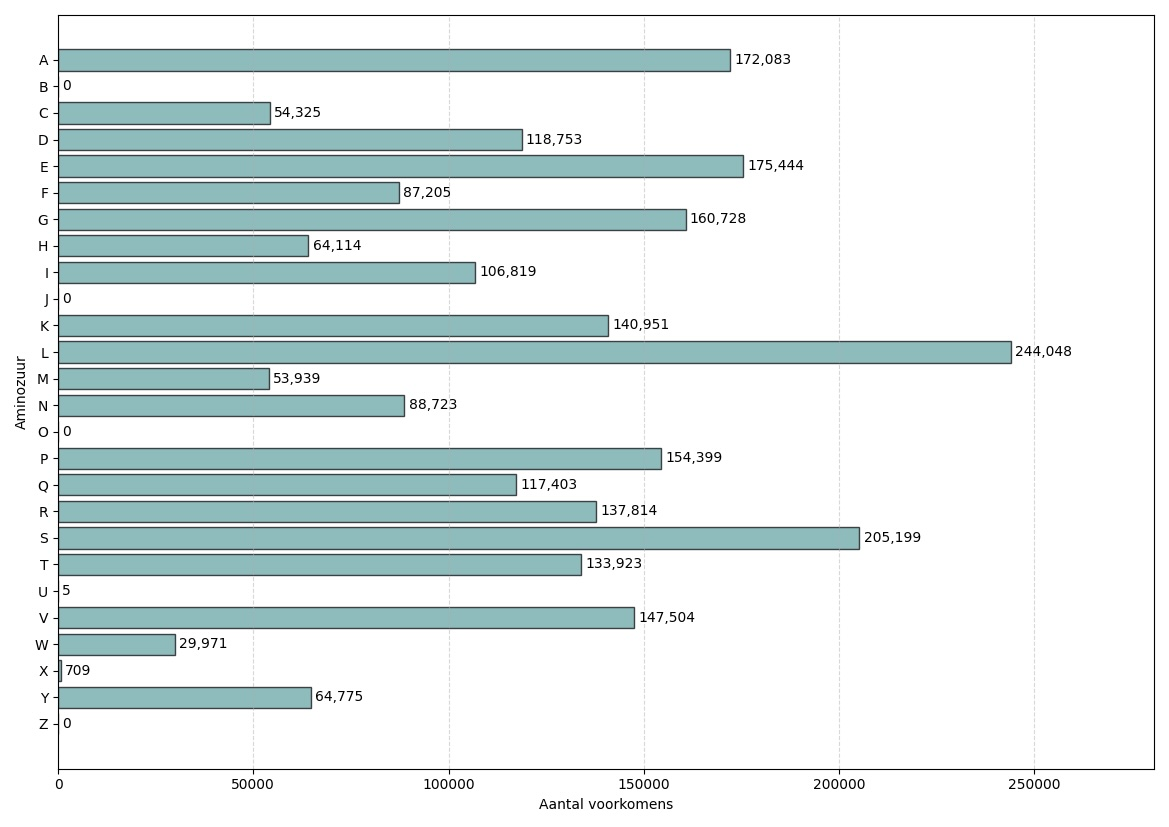
\includegraphics[width=0.485\linewidth]{humanprot_search_amino_acids}}
    \hfill
    \subfloat[Lengtedistributie van de peptiden in het Human-Prot zoekbestand]{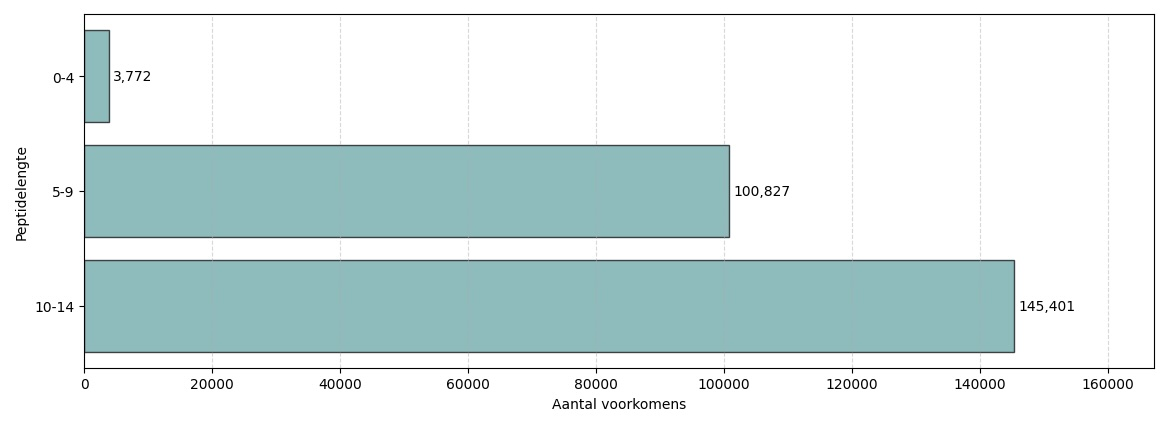
\includegraphics[width=0.485\linewidth]{humanprot_search_lengths}}
    \caption{Extra statistieken over het Human-Prot zoekbestand}\label{fig:humanprot_search_other_stats}
\end{figure}

\section{Swiss-Prot}\label{sec:swiss-prot-stats}
\begin{figure}[H]
    \centering
    \subfloat[Distributie van de aminozuren in het Swiss-Prot zoekbestand zonder \textit{missed cleavage}]{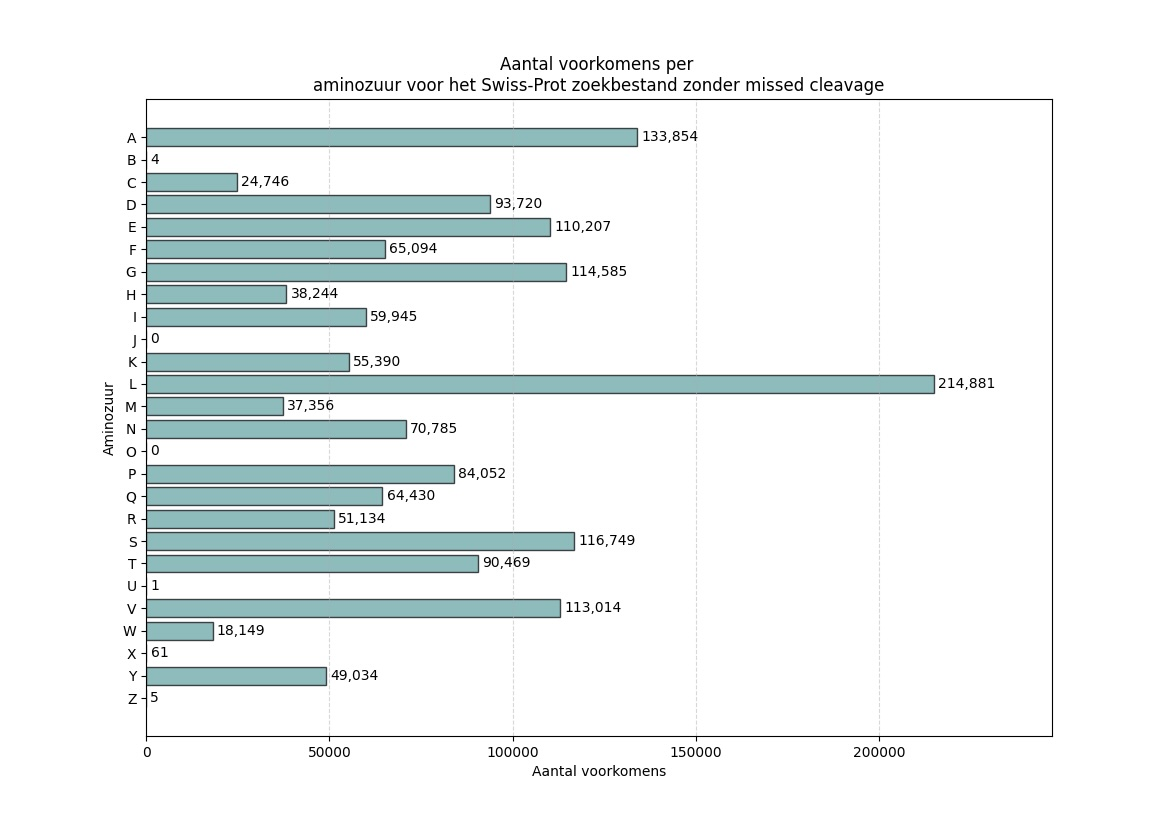
\includegraphics[width=0.485\linewidth]{swissprot_searchfile_no_missed_cleavage_amino_acids}}
    \hfill
    \subfloat[Lengtedistributie van de peptiden in het Swiss-Prot zoekbestand zonder \textit{missed cleavage}]{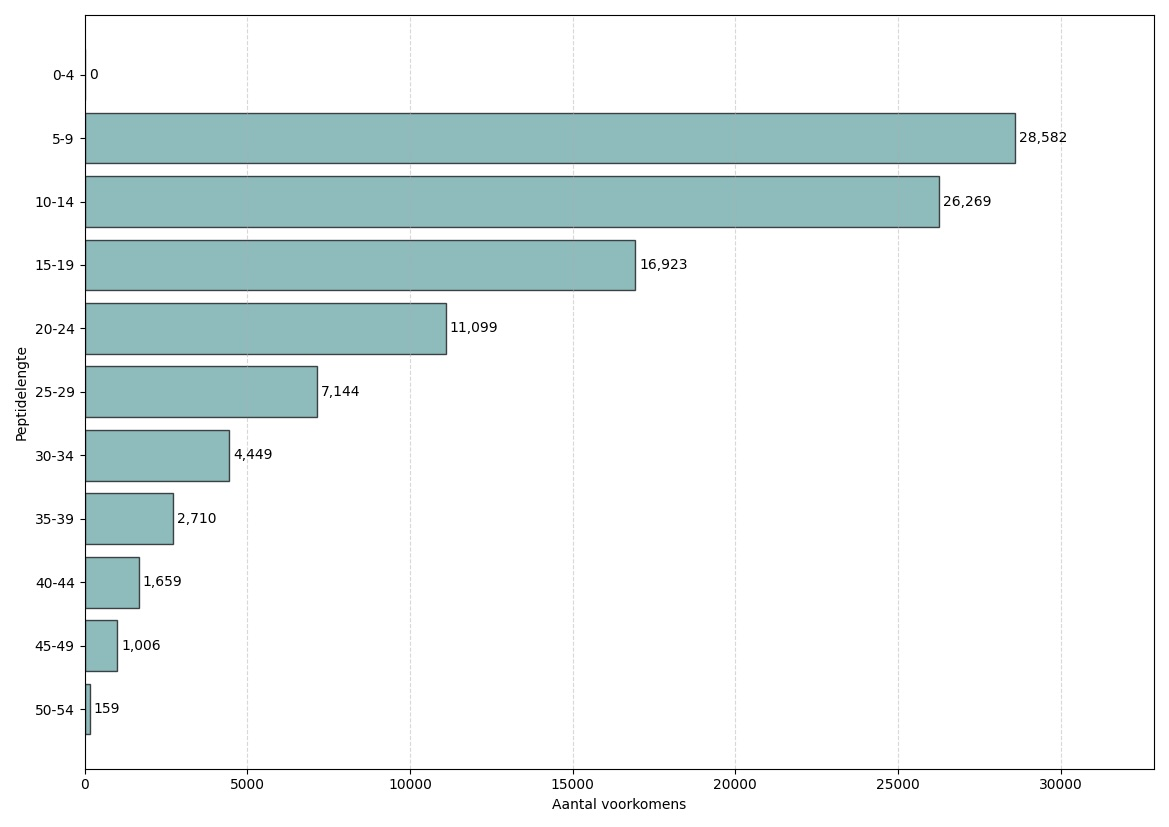
\includegraphics[width=0.485\linewidth]{swissprot_searchfile_no_missed_cleavage_lengths}}
    \caption{Extra statistieken over het Swiss-Prot zoekbestand zonder \textit{missed cleavage}}\label{fig:swissprot_search_no_missed_cleavage_other_stats}
\end{figure}
\begin{figure}[H]
    \centering
    \subfloat[Distributie van de aminozuren in het Swiss-Prot zoekbestand met \textit{missed cleavage}]{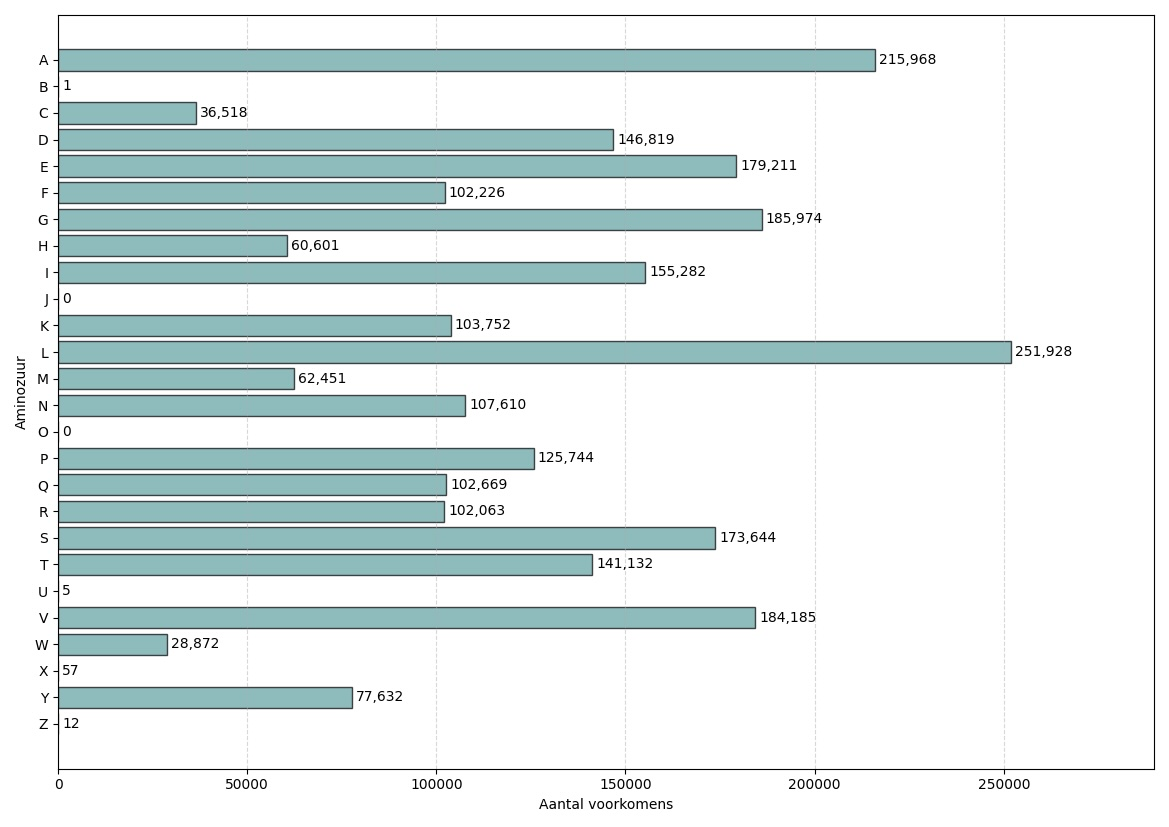
\includegraphics[width=0.485\linewidth]{swissprot_searchfile_missed_cleavage_amino_acids}}
    \hfill
    \subfloat[Lengtedistributie van de peptiden in het Swiss-Prot zoekbestand met \textit{missed cleavage}]{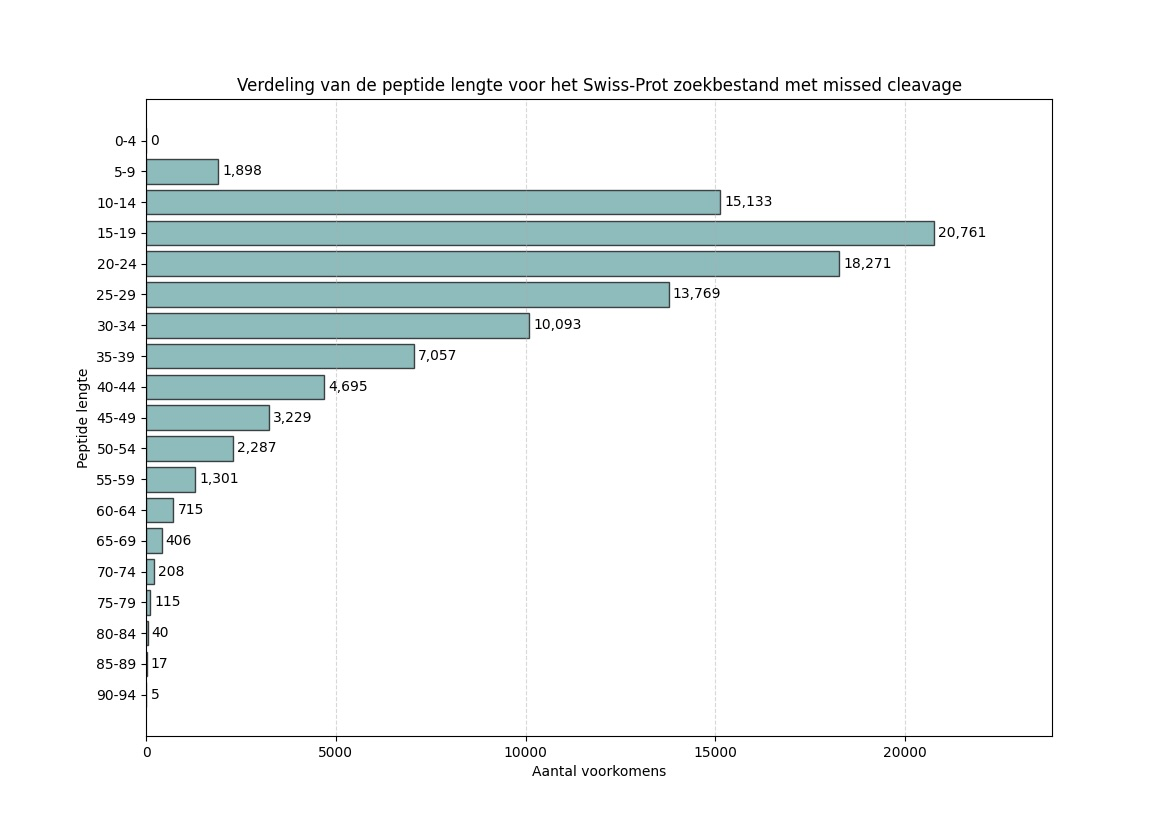
\includegraphics[width=0.485\linewidth]{swissprot_searchfile_missed_cleavage_lengths}}
    \caption{Extra statistieken over het Swiss-Prot zoekbestand met \textit{missed cleavage}}\label{fig:swissprot_search_missed_cleavage_other_stats}
\end{figure}

\section{SIHUMI}\label{sec:sihumi-stats}
\begin{figure}[H]
    \centering
    \subfloat[Distributie van de aminozuren in het SIHUMI S03 zoekbestand]{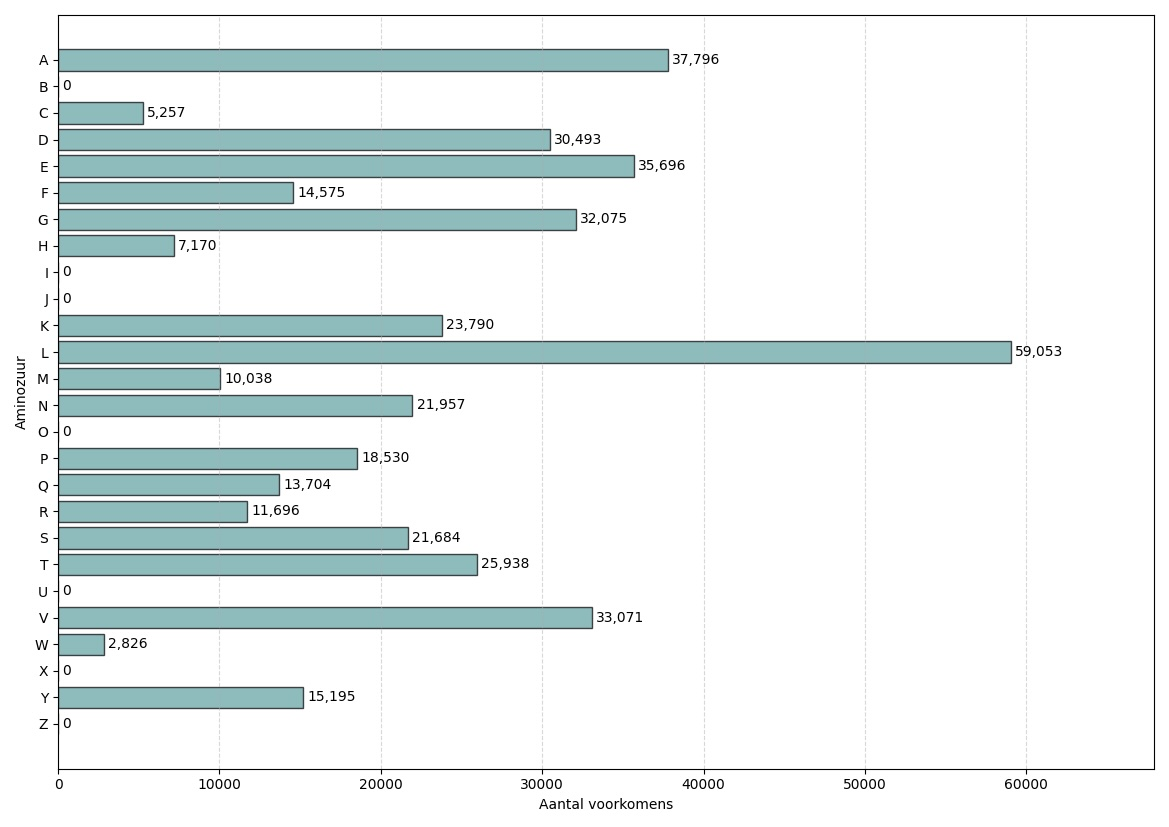
\includegraphics[width=0.485\linewidth]{sihumi_03_amino_acids}}
    \hfill
    \subfloat[Lengtedistributie van de peptiden in het in het SIHUMI S03 zoekbestand]{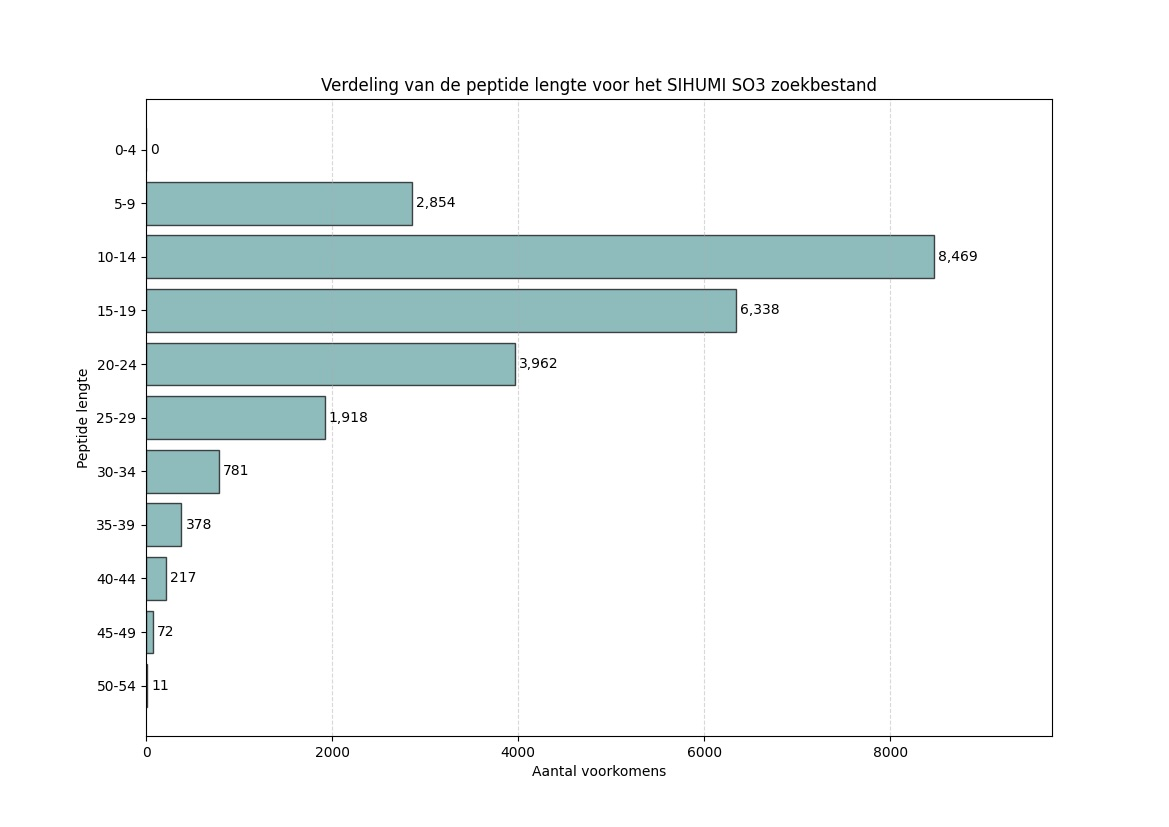
\includegraphics[width=0.485\linewidth]{sihumi_03_length}}
    \caption{Extra statistieken over het SIHUMI S03 zoekbestand}\label{fig:sihumi_03_other_stats}
\end{figure}
\begin{figure}[H]
    \centering
    \subfloat[Distributie van de aminozuren in het SIHUMI S05 zoekbestand]{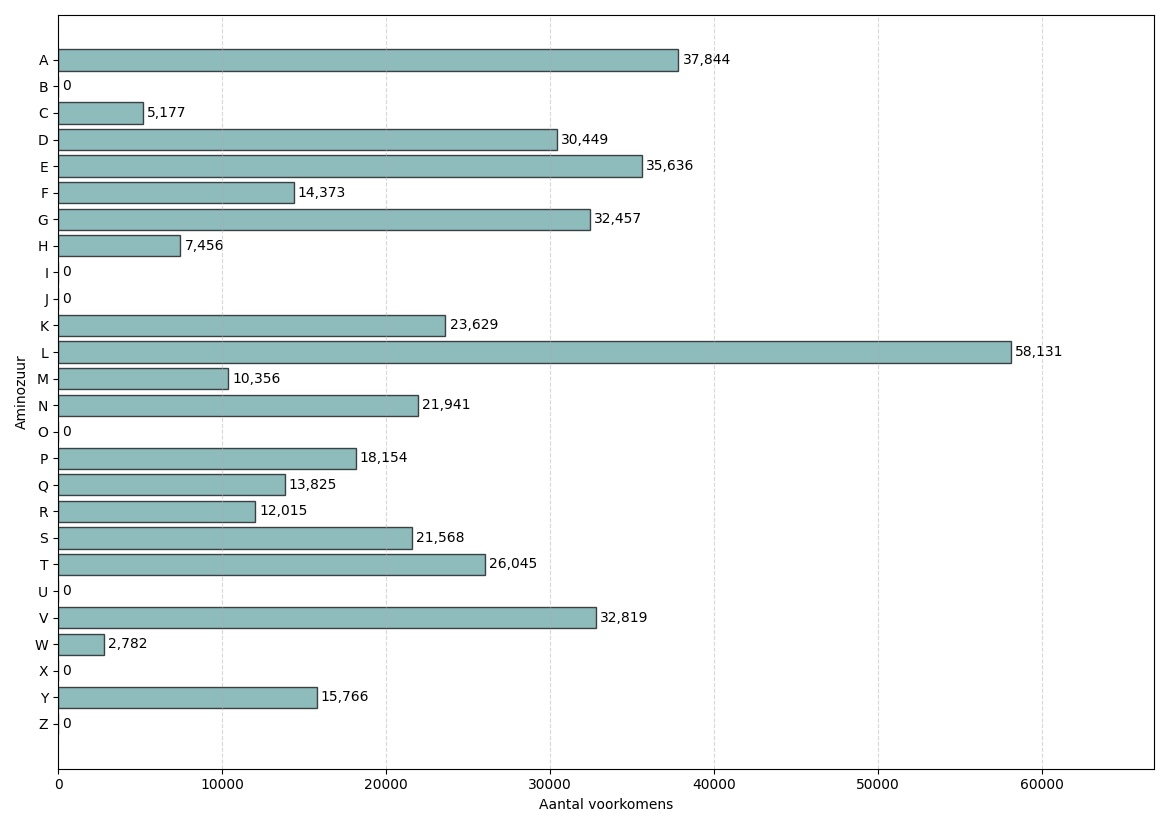
\includegraphics[width=0.485\linewidth]{sihumi_05_amino_acids}}
    \hfill
    \subfloat[Lengtedistributie van de peptiden in het in het SIHUMI S05 zoekbestand]{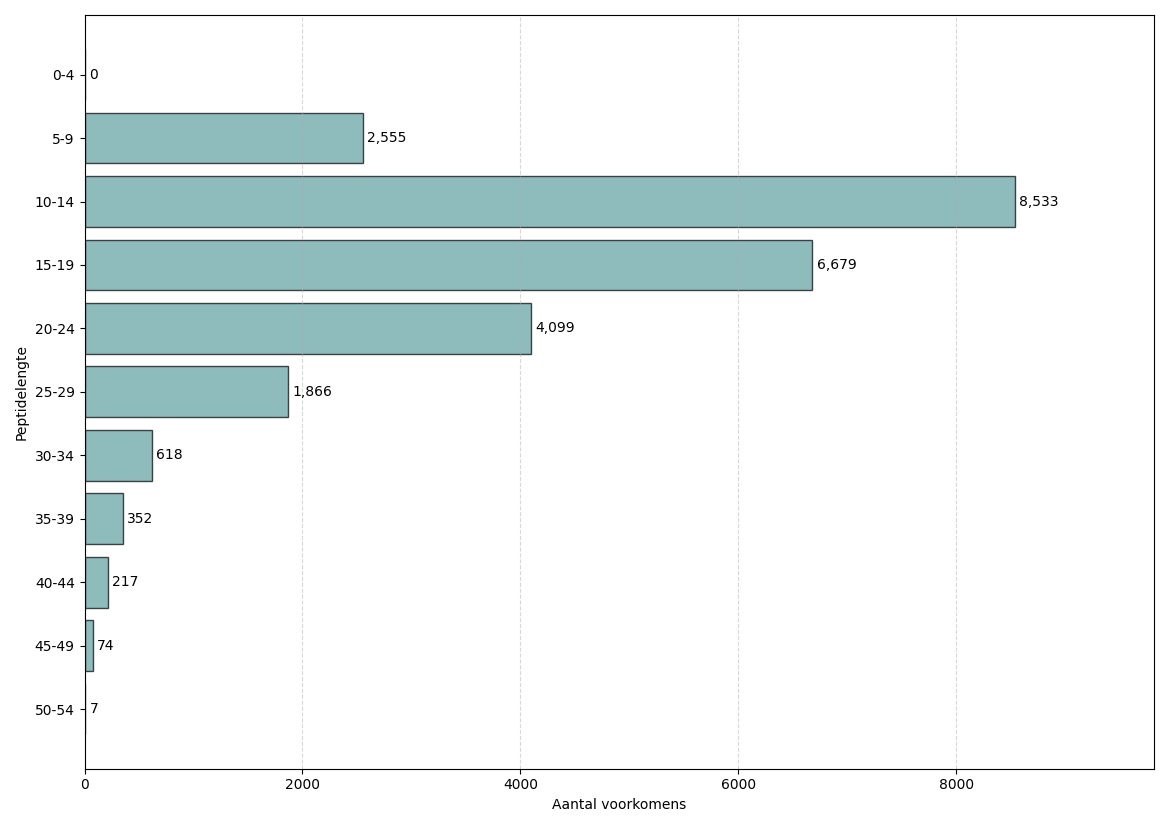
\includegraphics[width=0.485\linewidth]{sihumi_05_length}}
    \caption{Extra statistieken over het SIHUMI S05 zoekbestand}\label{fig:sihumi_05_other_stats}
\end{figure}
\begin{figure}[H]
    \centering
    \subfloat[Distributie van de aminozuren in het SIHUMI S07 zoekbestand]{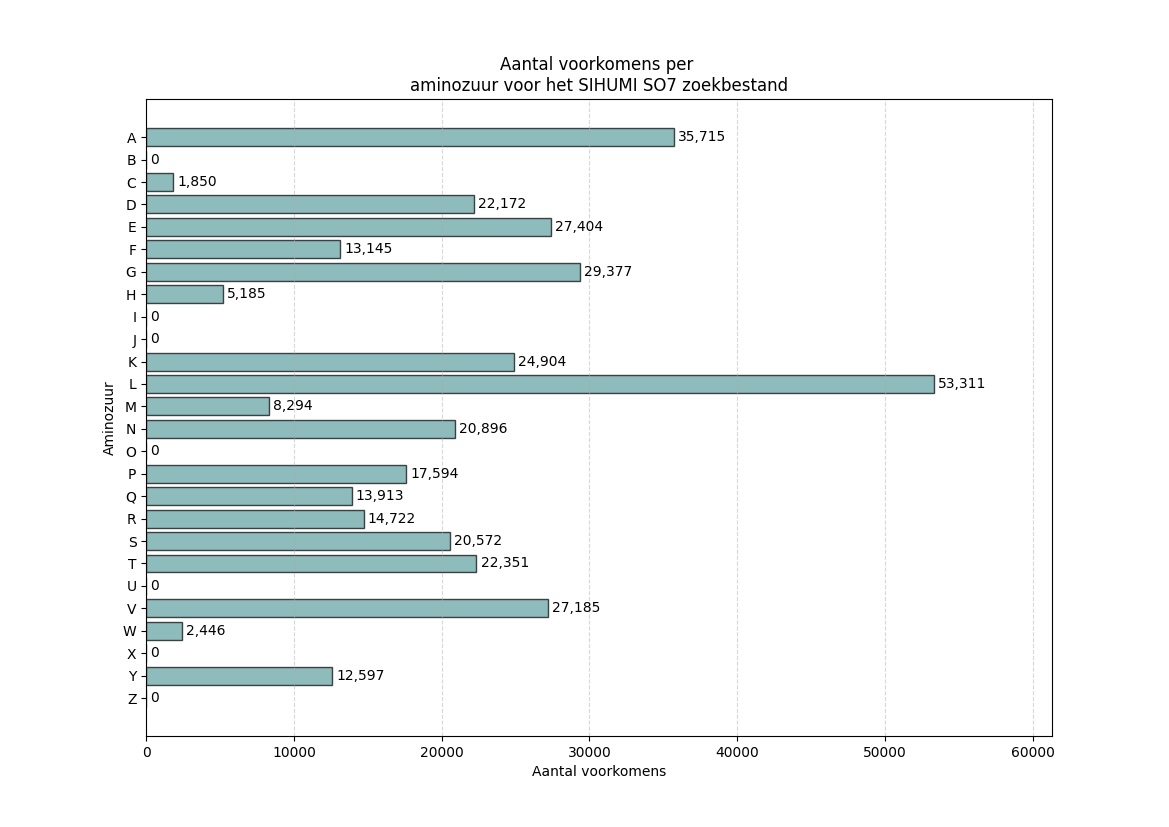
\includegraphics[width=0.485\linewidth]{sihumi_07_amino_acids}}
    \hfill
    \subfloat[Lengtedistributie van de peptiden in het in het SIHUMI S07 zoekbestand]{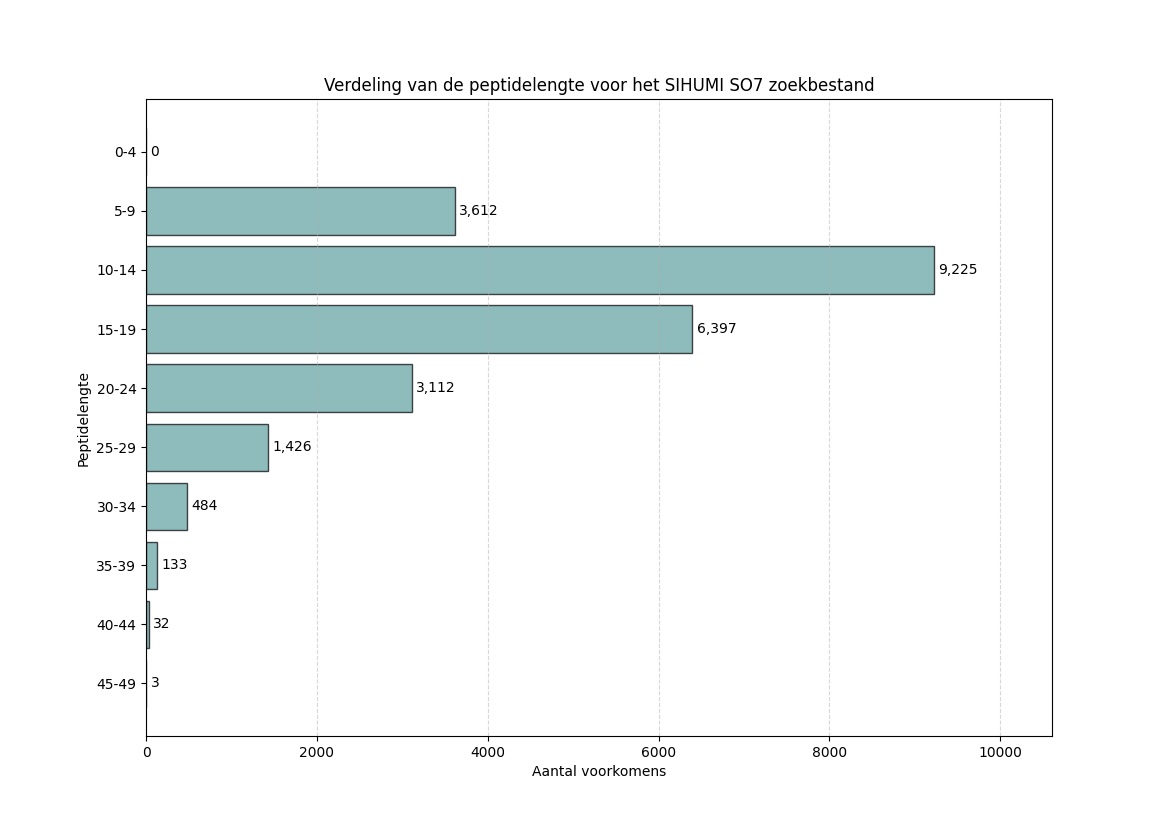
\includegraphics[width=0.485\linewidth]{sihumi_07_length}}
    \caption{Extra statistieken over het SIHUMI S07 zoekbestand}\label{fig:sihumi_07_other_stats}
\end{figure}
\begin{figure}[H]
    \centering
    \subfloat[Distributie van de aminozuren in het SIHUMI S08 zoekbestand]{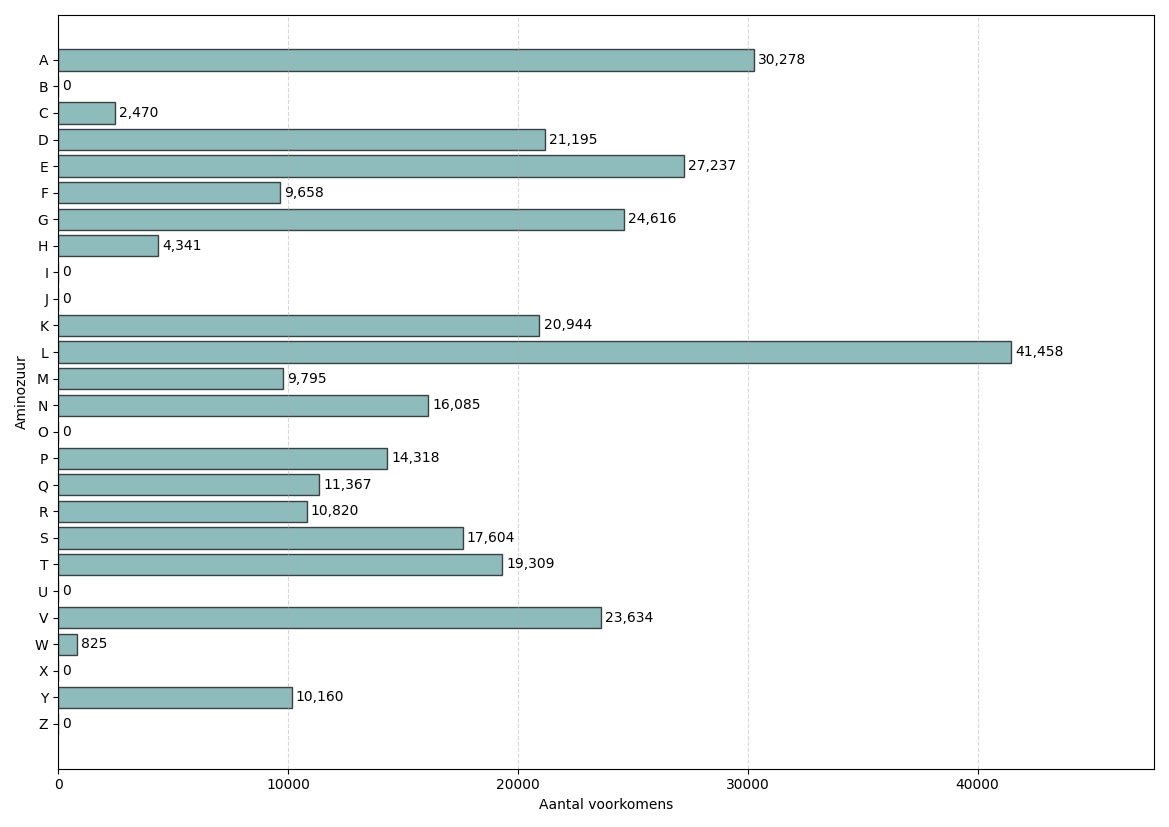
\includegraphics[width=0.485\linewidth]{sihumi_08_amino_acids}}
    \hfill
    \subfloat[Lengtedistributie van de peptiden in het in het SIHUMI S08 zoekbestand]{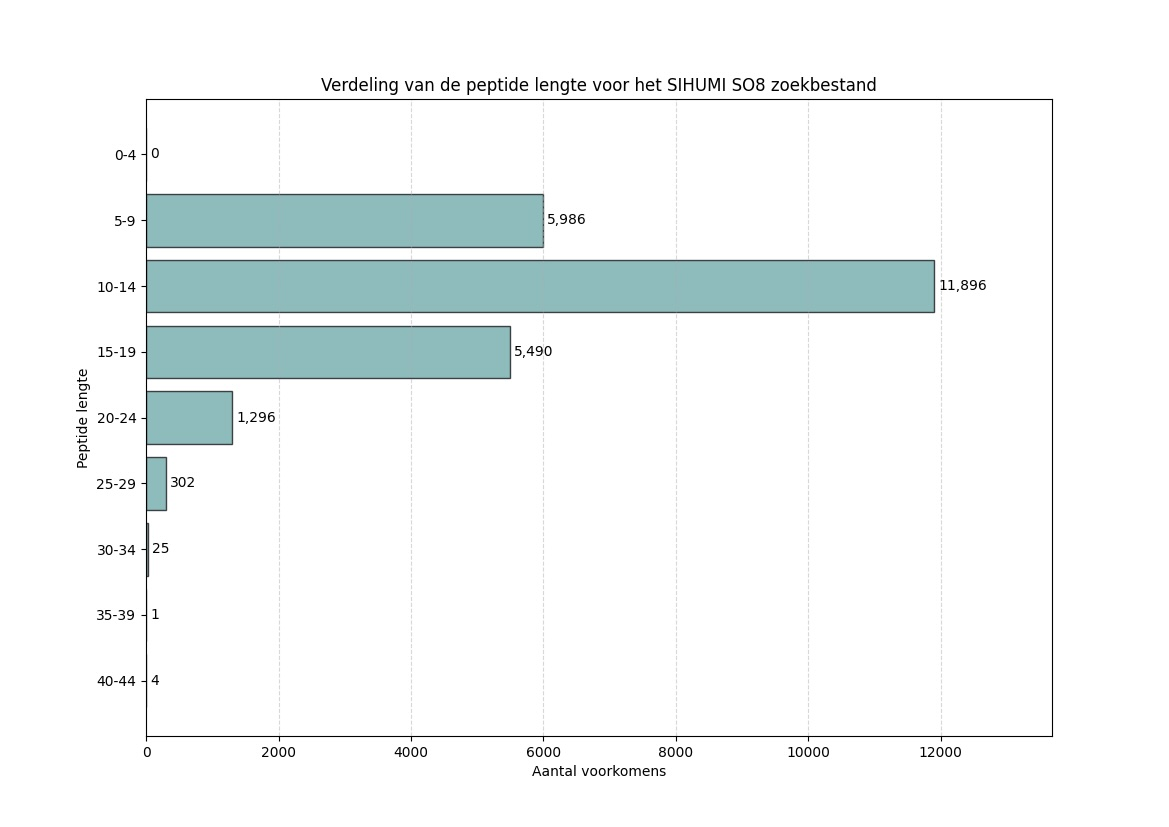
\includegraphics[width=0.485\linewidth]{sihumi_08_length}}
    \caption{Extra statistieken over het SIHUMI S08 zoekbestand}\label{fig:sihumi_08_other_stats}
\end{figure}
\begin{figure}[H]
    \centering
    \subfloat[Distributie van de aminozuren in het SIHUMI S11 zoekbestand]{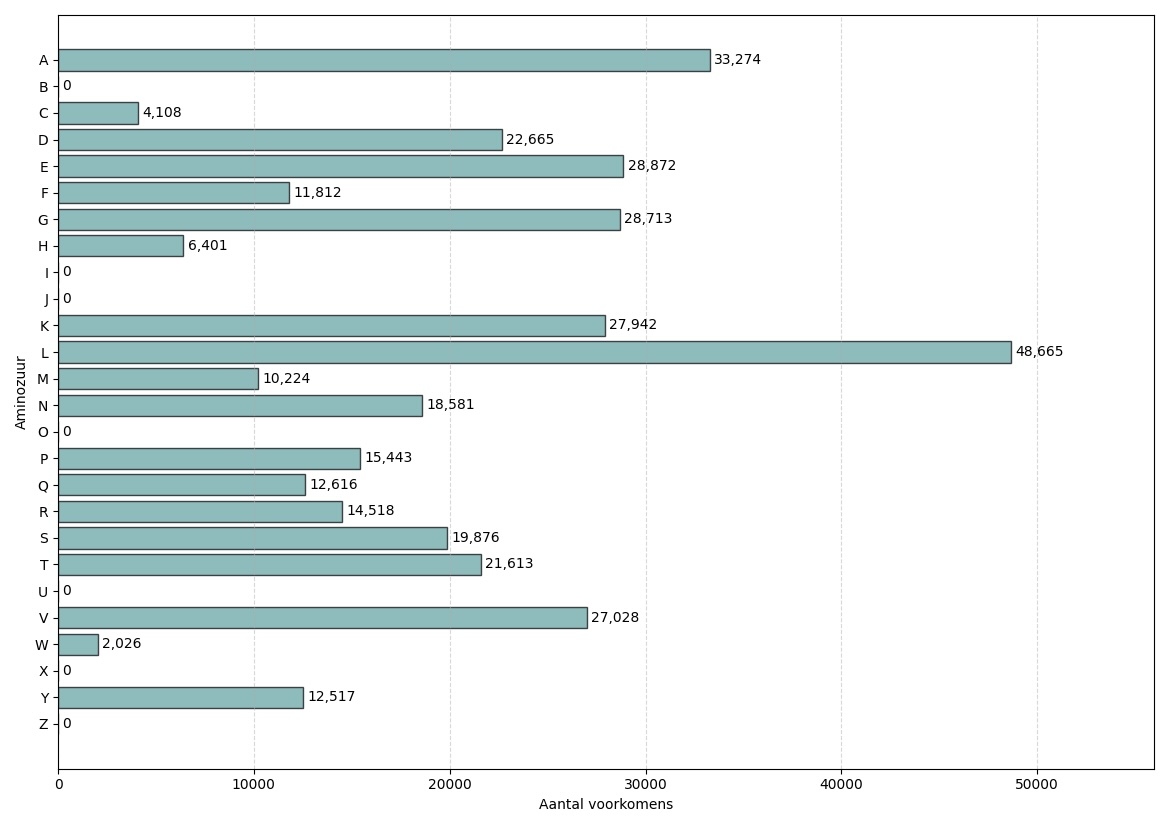
\includegraphics[width=0.485\linewidth]{sihumi_11_amino_acids}}
    \hfill
    \subfloat[Lengtedistributie van de peptiden in het in het SIHUMI S11 zoekbestand]{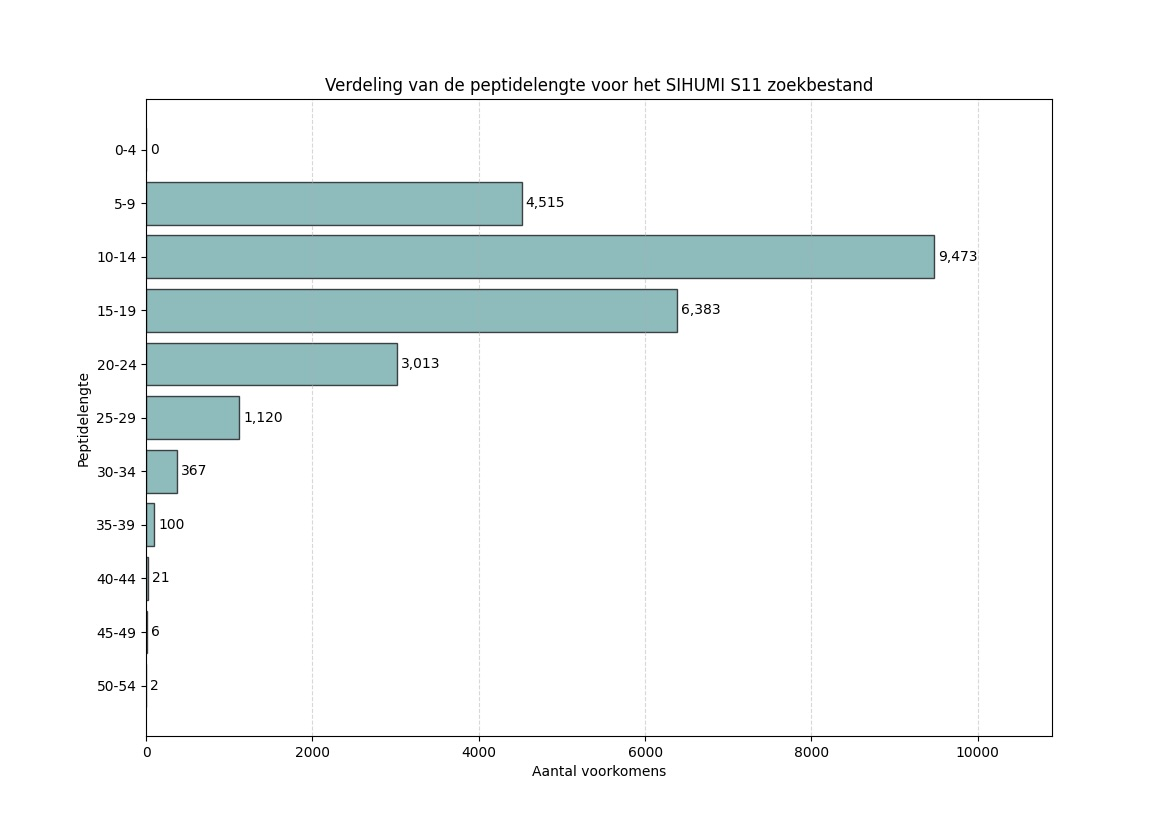
\includegraphics[width=0.485\linewidth]{sihumi_11_length}}
    \caption{Extra statistieken over het SIHUMI S11 zoekbestand}\label{fig:sihumi_11_other_stats}
\end{figure}
\begin{figure}[H]
    \centering
    \subfloat[Distributie van de aminozuren in het SIHUMI S14 zoekbestand]{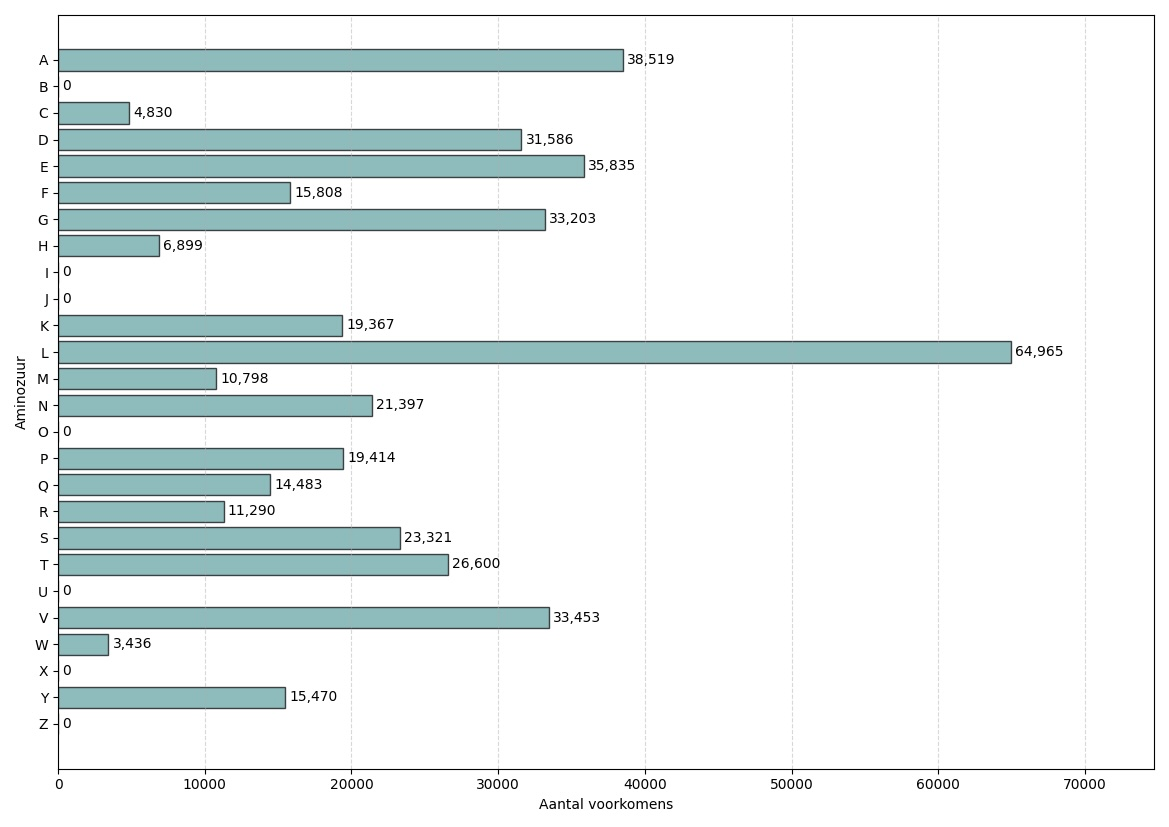
\includegraphics[width=0.485\linewidth]{sihumi_14_amino_acids}}
    \hfill
    \subfloat[Lengtedistributie van de peptiden in het in het SIHUMI S14 zoekbestand]{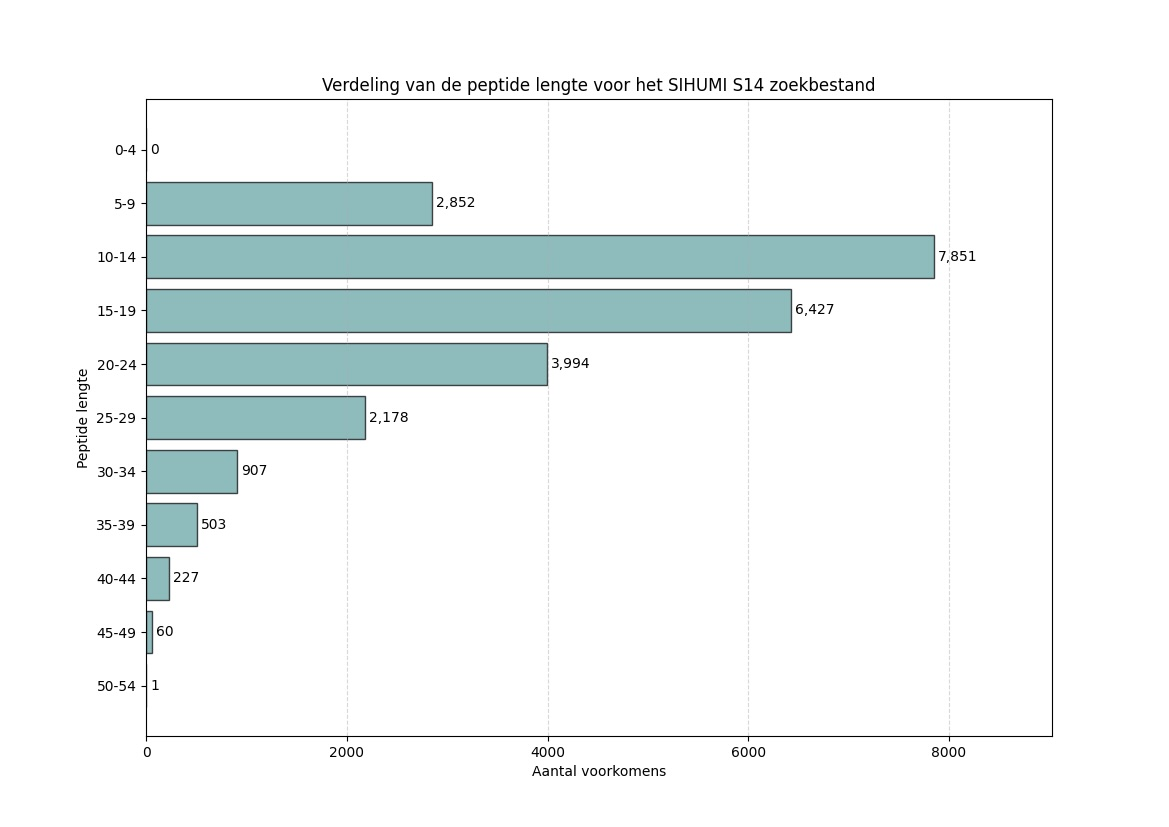
\includegraphics[width=0.485\linewidth]{sihumi_14_length}}
    \caption{Extra statistieken over het SIHUMI S14 zoekbestand}\label{fig:sihumi_14_other_stats}
\end{figure}